%\documentclass[10pt,final,journal]{IEEEtran}
%\documentclass[10pt,onecolumn,journal]{IEEEtran}
\documentclass[10pt,onecolumn,draftcls]{IEEEtran}
%\documentclass[10pt,final,journal]{IEEEtran}
%\documentclass[10pt,onecolumn,journal]{IEEEtran}
%\documentclass[10pt,onecolumn,draftcls]{IEEEtran}

\ifCLASSINFOpdf
\else
\fi

\usepackage{graphicx} 
\usepackage{amsthm}%proof 
\usepackage{amsmath} 
\usepackage{amsfonts} 
\usepackage{xcolor}
\graphicspath{{figures/}}
\newtheorem{myas}{Assumption}
\newtheorem{mydef}{Definition}
\newtheorem{mylem}{Lemma}
\newtheorem{myrem}{Remark}
\newtheorem{mythm}{Theorem}
\newtheorem{mycase_a}{Case}
\newtheorem{mycase_b}{Case} 
\newcommand\sgn{{\rm sgn}}
% there is only eq(27) need to cover two column
\newcommand{\NPL}[1]{\newcounter{mytempeqncnt}
\begin{figure*}[!t]
\normalsize
\setcounter{mytempeqncnt}{\value{equation}}
\setcounter{equation}{#1}}
\newcommand{\NPR}{\setcounter{equation}{\value{mytempeqncnt}}
\hrulefill
\vspace*{4pt}
\end{figure*}}

\hyphenation{op-tical net-works semi-conduc-tor}

\begin{document}

%\title{Discrete-time Sliding Mode Control for Deployment of Tethered Spacecraft System with Only Length and Angle Measurements}
\title{Discrete-time Sliding Mode Control for Deployment of Tethered Space Robot with Only Length and Angle Measurement}

\author{Zhiqiang~Ma,~\IEEEmembership{Member,~IEEE,}
        Panfeng~Huang,~\IEEEmembership{Senior~Member,~IEEE}
        %and~Jane~Doe,~\IEEEmembership{Life~Fellow,~IEEE}% <-this % stops a space
\thanks{This work was supported in part by the National Science Fund for Distinguished Young Scholars of China under Grant No. 61725303, in part by the National Natural Science Foundation of China under Grant No. 91848205 (Corresponding
author: Panfeng Huang).}

\thanks{Z. Ma and P. Huang are with National Key Laboratory of Aerospace Flight Dynamics and Research Center for Intelligent Robotics, School of Astronautics, Northwestern Polytechnical University, Xi'an 710072, China (zhiqiangma@nwpu.edu.cn, pfhuang@nwpu.edu.cn)}% <-this % stops a space
%\thanks{J. Doe and J. Doe are with Anonymous University.}% <-this % stops a space
\thanks{Manuscript received \today}
}
% The paper headers
\markboth{Journal of \LaTeX\ Class Files,~Vol.~14, No.~8, \today}%
{Shell \MakeLowercase{\textit{et al.}}: Bare Demo of IEEEtran.cls for IEEE Journals}

\maketitle

% As a general rule, do not put math, special symbols or citations
% in the abstract or keywords.
\begin{abstract}
% [purpose]
This paper proposes a nonlinear discrete-time sliding mode based tension control for deployment of tethered space robot with only length and angle measurements. 
% [Method]
The discrete-time dynamics of deployment is uncovered based on discretization of Hamilton’s principle. Taking into account the underactuated dynamics, the proposed discrete-time sliding surface can generate a specified reduced order  system which can be regarded as an uncertain discrete-time system with multiple time delays which is caused by a considerable sample interval, and the stability of reduced order  system is well analyzed by combining linear matrix inequation technique based on robust control theory and nonlinear discrete-time Lyapunov method. A novel input structure with the auxiliary variable sequence is presented to deal with the tension saturation, and the states can converge to the specified reduced order  system although the input saturation occurs. 
% [Result]
The proposed discrete-time method makes no appeal to velocity terms. It is cost-effective to use the proposed method for  the information of length and angle are easily measured rather than that of velocity, and it conduces to low requirements for the measurement ability of sensors.  
% [Conclusion]
Simulation results verify the stability analyses, and are coincident with the stability analyses.

\end{abstract}

% Note that keywords are not normally used for peerreview papers.
\begin{IEEEkeywords}
Discrete-time system, Discrete-time sliding mode control, Underactuated system, Tethered space robot, Input saturation.
\end{IEEEkeywords}






\IEEEpeerreviewmaketitle



\section{Introduction}

\IEEEPARstart{T}{ethered} space robot (TSR) are composed of terminal operation space robots and space tether, and it is appropriate for its distributed configuration to carry out  long-span space tasks of scientific detections and measurements on orbit~\cite{yu2018review}. 
Besides the mechanic design of TSR, the dynamics and control are also one of the most hot research spots recently, because TSR only uses tension of space tether to configure terminal operation space robots, which naturally performs coupled and underactuated dynamics~\cite{ma2017dynamic}. 
It is valuable to study these characteristics to enhance maneuver performance for specified space applications, such as debris capture and removal~\cite{wang2015coordinated,Zhang2017,Zhang2017JGCD,Huang2017,dai2018post} and orbital transfer~\cite{liu2017tether}.
Deployment of terminal operation space robot is typically employed in the fundamental phase of space task for subsequent detections or measurements, which is a key technique of space robot formation, and has been extensively studied recently~\cite{yu2017analytical,ma2018pure}.

Optimal control  is recognized strategy for deployment of TSR, and one of the most outstanding advantage is to regard the limited tension as a boundary condition to produce effective control commands~\cite{williams2008deployment,wen2008optimal}. 
Analytical methodology can maintain all nonlinear details to achieve stabilization of TSR, but it is a hard work to discover a stable structure and corresponding diffeomorphism~\cite{yu2017analytical}. 
Kang and Zhu reported an output feedback tension control based on energy to regulate the deployment, and pointed out that in existing methods the velocity terms usually act as the dissipation function to stabilize the closed-loop system, but from the practical perspective, it is easy to measure the length and angle rather than velocity measurement~\cite{Kang2018}.
Recently, variable structure control schemes were wildly used to study the deployment of TSR, and this methodology obtained well performance due to its insensitivity to disturbance~\cite{zhang2017adaptive}. Based on the knowledge of variable structure control, the switching control law divided entire system dynamics into two phases, namely, the reaching phase and the sliding phase, and the corresponding performances are determined by the design of switching law and sliding surface,  respectively~\cite{ma2017dynamic,ma2018pure}. Super-twisting sliding mode enhanced the ability of trivial sliding mode controllers for reaching the sliding surface, and it is hence adopted to stabilize the deployment of multiple space tethers for debris capture~\cite{Zhang2017JGCD}.

However, it is a matter of how we apply these theoretical control methods to the practical deployment of TSR, and there is a significant gap between the theoretical research and the applications. In present space engineering applications, the high-performance digital compute unit has been widely used and replaced the analog computer for the advantages of high integration density, ease maintenance and great flexibility. It is identified that digital-computer-based control systems require discrete-time control methods to satisfy the demand of high performance. However, it is worth noting that these methods mentioned above are in the view point of continuous-time system, and existing discrete-time methods for the deployment of TSR are rare. 

Normally, running a controller, which is designed based on continuous-time dynamics, will more or less affect the stability of control system, because the control performance of discrete-time system is evaluated by rise time and steady error related to the sample interval, and the interval time in continuous-time systems is identified as null~\cite{sun2018discrete}.  

Except the interval time, it is natural to adopt discrete-time control methods to synthesize an entire digital-computer-based engineering application for two reasons. The first one is that the stability analysis of discrete-time dynamics derives from digital-computer-based engineering process. Figure~\ref{fig:tetherreel} shows the schematic diagram of a classical engineering process for the tether winding of TSR, which extracts from winding mechanism for STARS of JAXA~\cite{Nohmi2009}, ATEx/STEX~\cite{Gates2001} and some other ground experiments~\cite{Iki2014,Nakaya2004}. This process starts from the sensor sampling the information of length and angle, and ends with the digital computer generating the command to control the winding mechanism. There is a problem that the continuous-time control command normally includes the velocity of length and angle,  and the velocity is not directly measured but calculated based on numerical method, such as the Euler difference or the numerical approximation~\cite{Kang2018}. But the difference method actively brings in the numerical error, which is not easy to analyze for its uncertainty, and will degenerate the control performance. 
This disadvantage can be dispelled by utilizing discrete-time method, because the discrete-time method is only comprised of position information, and the information contamination caused by Euler difference in continuous-time system can be avoided, leading to the deployment of TSR with only length and angle measurements, which aids dense mechanics and low mass in space missions. 
\begin{figure}[htbp]  
	\centering
\includegraphics[width=180pt]{tetherreel.eps}
\caption{Schematic diagram of tether reel mechanics with sensors} \label{fig:tetherreel}
\end{figure}  

As described above, discrete-time control methods conduce to the accurate command without the information uncertainty, and it is a more suitable implementation for the digital-computer-based system than continuous-time ones. However, it is an accompanying problem that all the existing continuous-time saturation strategy for the practical tension control can not directly work before modified. According to our knowledge, the studies on the discrete-time control method for the deployment of TSR are not abundant, neither are the achievements on discrete-time saturation strategies. 

Motivated by the points mentioned above, we proposed a new nonlinear discrete-time sliding mode control (DSMC) to stabilize the deployment motion of TSR. The novelties of this work contain: 
(1) it is the first sliding mode control to identify and characterize the role of sample interval in the deployment of TSR with only length and angle measurements; (2) the underactuated dynamics is insulated by the the specified sliding surface into the reduced order system, and the motion on the surface can divide the reduced order system into length part and swinging angle parts; (3) a novel auxiliary variable sequence is proposed for the purpose of eliminating the adverse impact from the input saturation.  

This paper is organized as follows: the first section reviews the recent research achievements on deployment of TSR, and Section~\ref{sec:Discrete-time Lagrangian} derives the discrete-time model of deployment of TSR based on discrete-time Lagrangian. Section~\ref{sec:Discrete-time Sliding Mode Control} presents the sliding surface and control command design, and corresponding stability analyses are also exhibited. Here also presents the auxiliary variable sequence for guaranteeing the establishment of sliding surface under saturated tension control. Simulation results are shown in Section~\ref{sec:Numerical Simulations} which verifies the stability analyses in previous sections.

\section{Discrete-time Lagrangian}\label{sec:Discrete-time Lagrangian} 
Discrete-time Lagrangian mechanics can be derived from discretization of Hamilton's principle that allows the methodology of variational integrators producing continuous-time analogue~\cite{Bloch2005Controlled}, 
and more detailed  variational approach to discrete mechanics can be seen in~\cite{Marsden2001Discrete}. 

As discussed in~\cite{Marsden2001Discrete}, a discrete-time Lagrangian is expressed by a map $L_d:Q\times Q\to \mathbb R$ where $Q\times Q$ is defined as discrete state space for state variable $q$. A key notation is that of the discrete-time mechanics, which is the time step $h\in \mathbb R$ referred as sample interval in digital computer control theory. Actually, $L_d:Q\times Q\times\mathbb R\to \mathbb R$ is dependent on time step. Define an increasing sequence involving time step $\left\{t_k=hk\left\vert k\in\mathbb N\right.\right\}\subset \mathbb R$, and construct the discrete-time path space to be~\cite{Marsden2001Discrete}.
\begin{align}
	C_d(Q)=\left\{q_d:\left\{t_k\right\}^N_{k=0}\to Q\right\}
\end{align}
A discrete-time trajectory $q_d=\left\{q_k\right\}^N_{k=0}$ belongs to $C_d(Q)$ with $q_k=q_d(t_k)$, and the discrete-time map is identified by
\begin{align}\label{eq:sd}
	S_d=\sum^{n-1}_{k=0}L_d(q_k,q_{k+1},h)
\end{align}
Computing the variational discretization of Eq.(\ref{eq:sd}) gives
\begin{align}\begin{split}\label{eq:dsd}
	&\delta S_d=\delta\sum^{n-1}_{k=0}L_d(q_k,q_{k+1},h)\\
	&=\sum^{n-1}_{k=0}\left[D_1L_d(q_k,q_{k+1},h)\delta q_k\right.\\
	&\quad\left.+D_2L_d(q_k,q_{k+1},h)\delta q_{k+1}\right]\\
	&=\sum^{n-1}_{k=1}\left[D_1L_d(q_k,q_{k+1},h)+D_2L_d(q_k,q_{k+1},h)\right]\delta q_{k}\\
		&\quad+D_1L_d(q_0,q_{1},h)\delta q_0+D_2L_d(q_{n-1},q_{n},h)\delta q_n
\end{split}\end{align}
where $D_{i}$ is the notation of discrete-time partial derivative, and $L_d$ can be obtained by combining time step $h$ and continuous-time Lagrange $L(q,\dot q)$~\cite{Marsden2001Discrete}
\begin{align}
	L_d(q_k,q_{k+1},h)=L(q,\dot q)
\end{align}
which is well known as the discrete Euler–Lagrange equations~\cite{Bloch2005Controlled}.

From the fact $\delta q_n=\delta q_0=0$ and $\delta S_d=0$~\cite{Marsden2001Discrete}, Eq.(\ref{eq:dsd}) can be rewritten as
\begin{align}\begin{split}
        \sum^{n-1}_{k=1}\left[D_1L_d(q_k,q_{k+1},h)+D_2L_d(q_k,q_{k+1},h)\right]\delta q_{k}=0
\end{split}\end{align} 

Considering  $\delta q_k\neq 0$, it is understood that the requirement on the establishment of the above equation is 
\begin{align}\label{eq:discrete EL}
	D_1L_d(q_k,q_{k+1},h)+D_2L_d(q_k,q_{k+1},h)=0
\end{align}
which is well known as the discrete-time Euler-Lagrangian, and $D_i$ is a symbol to indicate the discrete-time derivative with respect to the $i$th variable.

In what follows, we will first review the continuous-time Lagrangian mechanics of the deployment under some essential assumptions, and the relation between the discrete-time Lagrangian and the continuous-time Lagrangian will be introduced to aid the description of the discrete-time dynamics of deployment. Moreover, it is impossible for the tension control to stabilize the out-of-plane and in-plane dynamics simultaneously. The stability of out-of-plane dynamics is depended on the auxiliary thrusters, which can be controlled by conventional methods much easier than the tension for in-plane one, and we focus on the stability analyses of in-plane dynamics in this paper.  

We shall make two standing assumptions on the space tether and the orbit, and these assumptions will be needed throughout the paper.  
\begin{myas}
	During the deployment, it is assumed that the space tether is tensioned. Hence the tether can be regarded as a stick, and the entire system can be modelled as a `rolling dumbbell'.
\end{myas}
\begin{myas}
	It is required that the attitude of space platform will not be affected by the motion of terminal operation space robot, and the center of mass is running on a circular orbit.
\end{myas}

Under the assumptions mentioned above, considering the continuous-time Lagrangian of deployment dynamics on circular orbit, the kinetic and potential energy can be respectively expressed by
	\begin{align}\begin{split}
	T&=\frac{1}{2}\bar m\Omega^2R_0^2+\frac{1}{2}\bar{m}l^2(\theta'+\Omega)^2+\frac{1}{2}\bar{m}l'^2\\
	V&=-\bar m\Omega^2R^2_0+\frac{1}{2}\bar{m}\Omega^2l^2[1-3\cos^2\theta]
	\end{split}\end{align}
	where $m=m_1+m_2$ is the total mass of system, and $\bar m=m_1m_2/(m_1+m_2)$ with $m_1$ and $m_2$ being mass of space platform and terminal operation robot, respectively. $\Omega$ represents orbital angular velocity, and $R_0$ denotes the distance from the earth's core to the centroid of system. $l$ is the length of space tether, and $\theta$ is in-plane swinging angle. 
	
	Subtract $V$ from $T$ to obtain $L=T-V$ as follows 
	\begin{align*}
		L&=\frac{3}{2}\bar m\Omega^2R_0^2+\frac{1}{2}\bar{m}l^2(\theta'+\Omega)^2+\frac{1}{2}\bar{m}l'^2\\
		&\quad-\frac{1}{2}\bar{m}\Omega^2l^2(1-3\cos^2\theta)
	\end{align*}

	Select generalized coordinate variable $q=(\theta,l)$ and taking forward Euler discretization with $\phi_k=(\theta_k,l_k,\theta_{k+1},l_{k+1})$, and the discrete-time Lagrangian follows
 % \begin{widetext}

  %\leftsep
%\NPL
  \begin{align*}
	&L_d(\phi_k,h)=L\left[\theta_k,l_k,(\theta_{k+1}-\theta_{k})/h,(l_{k+1}-l_{k})/h\right]\\
		&=\frac{3}{2}\bar m\Omega^2R_0^2+\frac{1}{2}\bar{m}l_k^2\left(\frac{\theta_{k+1}-\theta_k}{h}+\Omega\right)^2\\
		&\quad+\frac{1}{2}\bar{m}\left(\frac{l_{k+1}-l_k}{h}\right)^2-\frac{1}{2}\bar{m}\Omega^2l_k^2(1-3\cos^2\theta_k)
	\end{align*}\begin{align*}
			&L_d(\phi_{k-1},h)=L\left[\theta_{k-1},l_{k-1},(\theta_{k}-\theta_{k-1})/h,(l_{k}-l_{k-1})/h\right]\\
		&=\frac{3}{2}\bar m\Omega^2R_0^2+\frac{1}{2}\bar{m}l_{k-1}^2\left(\frac{\theta_{k}-\theta_{k-1}}{h}+\Omega\right)^2\\
		&\quad+\frac{1}{2}\bar{m}\left(\frac{l_{k}-l_{k-1}}{h}\right)^2-\frac{1}{2}\bar{m}\Omega^2l_{k-1}^2(1-3\cos^2\theta_{k-1})
  \end{align*}
 
%\NPR
	According to discrete-time Euler-Lagrange mechanics, one has
	\begin{align}\begin{split}
	&D_1L_d(\phi_k,h)+D_3L_d(\phi_{k-1},h)=Q_k\\
	&D_2L_d(\phi_k,h)+D_4L_d(\phi_{k-1},h)=u_k
	\end{split}\end{align}
	where
	\begin{align}\begin{split}
		&D_1L_d(\phi_k,h)=\frac{\partial L_d(\phi_k,h)}{\partial \theta_k}\\
		&=\bar{m}l_k^2\left(\frac{\theta_{k}}{h^2}-\frac{\theta_{k+1}}{h^2}-\frac{\Omega}{h}\right)-3\bar{m}\Omega^2l^2_k\cos\theta_{k}\sin\theta_{k}\\
		&D_2L_d(\phi_k,h)=\frac{\partial L_d(\phi_k,h)}{\partial l_k}\\
		&=\bar{m}l_k\left(\frac{\theta_{k+1}-\theta_{k}}{h}+\Omega\right)^2+\frac{\bar{m}l_k}{h^2}\\
		&\quad-\frac{\bar{m}l_{k+1}}{h^2}-\bar{m}\Omega^2l_k(1-3\cos^2\theta_{k})\\
		&D_3L_d(\phi_{k-1},h)=\frac{\partial L_d(\phi_{k-1},h)}{\partial \theta_k}\\
		&=\bar{m}l^2_{k-1}\left(\frac{\theta_{k}}{h^2}-\frac{\theta_{k-1}}{h^2}+\frac{\Omega}{h}\right)\\
		&D_4L_d(\phi_{k-1},h)=\frac{\partial L_d(\phi_{k-1},h)}{\partial l_k}
		=\frac{\bar{m}(l_k-l_{k-1})}{h^2}
	\end{split}\end{align}
	and $u_k=-\tau_k< 0$ is the inverse tension at time $t_k$. We use the symbol $Q_k$ to denote the generalized force directly drives the dynamics of swinging angle at time $t_k$, and we select $Q_k=0$ to construct an discrete-time underactuated deployment dynamics under the pure tension control. 
	
	The discrete-time dynamics of deployment can be expressed by the following iteration action
	\begin{align}\begin{split}\label{eq:theta_k+1}
		\theta_{k+1}=&\left(\theta_{k}-h\Omega\right)+\frac{l^2_{k-1}}{l^2_k}\left(\theta_{k}-\theta_{k-1}+h\Omega\right)\\
		&-3h^2\Omega^2\cos\theta_{k}\sin\theta_{k}\\
		l_{k+1}=&l_kh^2\left(\frac{\theta_{k+1}-\theta_{k}}{h}+\Omega\right)^2+l_k+(l_k-l_{k-1})\\
		&-h^2\Omega^2l_k(1-3\cos^2\theta_{k})+\frac{h^2u_k}{\bar{m}}
	\end{split}\end{align}
	
	Introducing $\lambda_k=l_k/L-1$ into the above equations, where $L$ is the total length of space tether, leads to dynamics with dimensionless length 
	\begin{align}\begin{split}\label{eq:lambda_k+1}
		\theta_{k+1}&=\left(\theta_{k}-h\Omega\right)+\frac{(\lambda_{k-1}+1)^2}{(\lambda_k+1)^2}\left(\theta_{k}-\theta_{k-1}+h\Omega\right)\\
		&\quad-3h^2\Omega^2\cos\theta_{k}\sin\theta_{k}\\
		\lambda_{k+1}&=(\lambda_k+1)h^2\left(\frac{\theta_{k+1}-\theta_{k}}{h}+\Omega\right)^2+2\lambda_k-\lambda_{k-1}\\
		&\quad-h^2\Omega^2(\lambda_k+1)(1-3\cos^2\theta_{k})+\frac{h^2u_k}{\bar{m}L}
	\end{split}\end{align}
	\begin{myrem}\label{remark:1}
		Physically, the deployed tether is shorter than the desired total length, and it is often rephrased as $\lambda\in(-1,0]$. It is for avoiding colliding that $\lambda>-1$ during the deployment mission. From Eq.(\ref{eq:theta_k+1}) to Eq.(\ref{eq:lambda_k+1}), it is understood that $\theta_{k+1}$ is dependent on $\theta$ and $\lambda$ at time $t_k$ and $t_{k-1}$, and $\lambda_{k+1}$ is moreover related to $\theta$ at $t_{k+1}$. Hence, it is required for the discrete-time numerical simulation and experiment to iterate $\theta$ before calculating $\lambda$ in a sample period.
        \end{myrem}
        \section{Discrete-time Sliding Mode Control}\label{sec:Discrete-time Sliding Mode Control} 
	Sliding surface is a manifold which attracts trajectories to converge onto and stay there. In this section, we will firstly introduce a nonlinear discrete-time sliding surface, and then drive the states onto the sliding surface via the trivial switching law with the equivalent technique.

	Selecting nonlinear discrete-time sliding surface $s(k)$:
	\begin{align}\begin{split}\label{eq:discrete time sliding furface}
				s(k) &= c_2\theta_{k-1}h^2\Omega^2+c_1(\theta_k-\theta_{k-1})h\Omega\\
				&\quad-\frac{2(\lambda_k-\lambda_{k-1})(h\Omega+\theta_k-\theta_{k-1})}{\lambda_{k-1}+1}\\
		&\quad-3h^2\Omega^2\cos\theta_{k-1}\sin\theta_{k-1}-\alpha\lambda_{k-1}h^2\Omega^2
	\end{split}\end{align}
	where $c_1>0$, $c_2>0$ and $\alpha>0$ are all controller parameters.

	To deduce the reaching condition of sliding surface, we begin by taking the forward Euler difference of $s(k)$ to get
	\begin{align*}\begin{split}
                &[s(k+1)-s(k)]/h\\
                &=c_2(\theta_k-\theta_{k-1})h\Omega^2+c_1[(\theta_{k+1}-\theta_k)-(\theta_{k}-\theta_{k-1})]\Omega\\
                &\quad-3h\Omega^2(\cos\theta_k\sin\theta_k-\cos\theta_{k-1}\sin\theta_{k-1})\\
				&\quad-\alpha(\lambda_k-\lambda_{k-1})h\Omega^2+\frac{2(\lambda_k-\lambda_{k-1})(h\Omega+\theta_k-\theta_{k-1})}{(\lambda_{k-1}+1)h}\\
				&\quad+\frac{2(\lambda_k-\lambda_{k+1})(h\Omega+\theta_{k+1}-\theta_{k})}{(\lambda_{k}+1)h}
        \end{split}\end{align*}
        \begin{align*}\begin{split}
                &\Rightarrow s(k+1)-s(k)\\
                &=c_2(\theta_k-\theta_{k-1})h^2\Omega^2+c_1[(\theta_{k+1}-\theta_k)-(\theta_{k}-\theta_{k-1})]h\Omega\\
				&\quad-3h^2\Omega^2(\cos\theta_k\sin\theta_k-\cos\theta_{k-1}\sin\theta_{k-1})\\
				&\quad-\alpha(\lambda_k-\lambda_{k-1})h^2\Omega^2+\frac{2(\lambda_k-\lambda_{k-1})(h\Omega+\theta_k-\theta_{k-1})}{(\lambda_{k-1}+1)}\\
                &\quad+\frac{2(\lambda_k-\lambda_{k+1})(h\Omega+\theta_{k+1}-\theta_{k})}{(\lambda_{k}+1)}
	\end{split}\end{align*} 
	Rewrite Eq.(\ref{eq:lambda_k+1})
	\begin{align}\begin{split}
                \lambda_{k+1}&=(\lambda_k+1)h^2\left(\frac{\theta_{k+1}-\theta_{k}}{h}+\Omega\right)^2
                -\lambda_{k-1}\\
                &\quad+2\lambda_k-h^2\Omega^2(\lambda_k+1)(1-3\cos^2\theta_{k})+bu(k)
	\end{split}\end{align}
	with $b = \frac{h^2}{\bar{m}L}$.
	
	Accordingly $s(k+1)-s(k)$ can be described by 
	\begin{align} \label{eq:sk+1-sk}
		s(k+1)-s(k)=\Phi_1(k)+\Phi_3(k)(\Phi_2(k)+bu(k))
	\end{align}
	where 
	\begin{align}\begin{split}
		&\Phi_1(k)
				=c_2(\theta_k-\theta_{k-1})h^2\Omega^2\\
				&\quad+c_1[(\theta_{k+1}-\theta_k)-(\theta_{k}-\theta_{k-1})]h\Omega\\
                &\quad-3h^2\Omega^2(\cos\theta_k\sin\theta_k-\cos\theta_{k-1}\sin\theta_{k-1})\\
				&\quad-\alpha(\lambda_k-\lambda_{k-1})h^2\Omega^2+\frac{2\lambda_k(h\Omega+\theta_{k+1}-\theta_{k})}{(\lambda_{k}+1)}\\
				&\quad+\frac{2(\lambda_k-\lambda_{k-1})(h\Omega+\theta_k-\theta_{k-1})}{(\lambda_{k-1}+1)}\\
				&\Phi_2(k)=(\lambda_k+1)h^2\left(\frac{\theta_{k+1}-\theta_{k}}{h}+\Omega\right)^2\\
				&\quad+2\lambda_k-\lambda_{k-1}-h^2\Omega^2(\lambda_k+1)(1-3\cos^2\theta_{k})\\
				&\Phi_3(k)=-\frac{2(h\Omega+\theta_{k+1}-\theta_{k})}{(\lambda_{k}+1)}
	\end{split}\end{align}

	Based on the equivalent control technique, the input $u(k)=u_{eq}(k)+u_{sw}(k)$ can be designed to fulfill the reaching condition of sliding surface
	\begin{align}\begin{split}\label{eq:control law}
		u_{eq}(k) &= -\left(\frac{\Phi_1(k)}{b\Phi_3(k)}+\frac{\Phi_2(k)}{b}\right)\\
		u_{sw}(k) &= -\frac{\eta s(k)}{b\Phi_3(k)}
	\end{split}\end{align}
	
	Substituting the input in Eq.(\ref{eq:control law}) into Eq.(\ref{eq:sk+1-sk}) yields the following derivation 
	\begin{align}\begin{split}\label{eq:s(k+1)-s(k) s}
		&s(k+1)-s(k) = -\eta s(k)\\
		\Rightarrow &s(k+1)=(1-\eta)s(k)\\
		\Rightarrow &s(k)=(1-\eta)^ks(0)
	\end{split}\end{align}

	If $\eta$ is chosen to satiety $\eta\in(0,2)$, then $s(k)=0$ is asymptotically stable with $k\to\infty$. 
	
	Alternatively, one can select a trivial relay switching input constructed with the sign function.
	\begin{align}
		u_{sw}(k) &= -\frac{\eta \sgn \left[s(k)\right]}{b\Phi_3(k)}
	\end{align}

	Under the control with above switching input, the derivation process from Eq.(\ref{eq:sk+1-sk}) to Eq.(\ref{eq:s(k+1)-s(k) s}) can be updated as
	\begin{align}\begin{split}\label{eq:s(k+1)-s(k)}
		s(k+1)-s(k) &= -\eta \sgn\left[s(k)\right]\\
		s(k+1)+s(k) &= -\eta \sgn\left[s(k)\right]+2s(k)\\
		s^2(k+1)-s^2(k) &= -2\eta\vert s(k)\vert+\eta^2\\
		&=-2\eta\left(\vert s(k)\vert-\eta/2\right)
	\end{split}\end{align}

	Considering a set $\Theta=\left\{x\left\vert x<\eta,x\in \mathbb{R}\right.\right\}$, if $s(0)\notin\Theta$ and $s(k)$ enters $\Theta$ for the first time at step $\xi+1$ , it is easy to calculate the reaching step of sliding surface according to the following inequation 
	\begin{align}\label{eq:eta s}
		\eta^2-s^2(0)\le s^2(\xi)-s^2(0)\le -\xi\eta^2
	\end{align}
	The reaching step is related to the initial $s(0)$ and the control parameter $\eta$, and can be expressed by $\xi\le\frac{s^2(0)-\eta^2}{\eta^2}$.
	\begin{myrem}
		This section provides two switching inputs to drive $s(k)$ onto the discrete-time sliding surface $s(k)=0$. It firstly gives an analysis on the asymptotical stability under the proportional switching input, and it implies $s(k)\to 0$ with $k\to\infty$. The relay switching input is characterized by reaching the sliding surface in finite step, which indicates that $s(k)$ enters a boundary layer $\Theta=\left\{x\left\vert x<\eta,x\in \mathbb{R}\right.\right\}$. 
		
		 From Eq.(\ref{eq:eta s}), the surface variable $s(k)$ spends $\xi$ steps to enter the set $\Theta$, and $\xi$ is a natural number if and only if Eq.(\ref{eq:eta s}) holds. Hence, it is required that $\eta$ should be selected smaller than $\vert s(0)\vert$, namely, $\eta<\vert s(0)\vert$, which implies that the selection of $\eta$ is determined by the initial states since $s(0)$ is composed of the initial conditions as shown in Eq.(\ref{eq:discrete time sliding furface}).
		
		The following stability analyses on the sliding surface are dependent on the availability of sliding surface, and in subsection~\ref{subsec:rssa} and~\ref{subsec:astl}, we will analyze the stability of reduced order system under the assumption that the asymptotical stability of $s(k)=0$ holds for the sake of simplification and clarity.
	\end{myrem}
	%\subsection{Input constraint}

	%Previous section presents a tension control law for deployment without input constraint considered, and physically, tension is critically positive due to its tensile property, which is worth being taken into account.

	%Considering the following relation expressing the tension constraint
	%\begin{align}
	%	\underline  u(k) =u(k)-\bar u(k)
	%\end{align}
	%where $\underline  u(k)<0$ is a tension input, and $u(k)$ is the command generated from the controller mentioned in last section. When $u(k)<0$ is a proper tension command, $\bar u(k)=0$, and conversely when $u(k)\ge 0$, which should be saturated to ensure the tension existing, $\bar u(k)>0$. Rewriting Eq.(\ref{eq:s(k+1)-s(k)}) with $\underline  u(k)$ and $\Delta(k) =b\bar  u(k)$, one has
	%\begin{align}\begin{split}
	%	s(k+1)-s(k) =& -\eta \sgn\left[s(k)\right]-\Delta(k)\\
	%	s(k+1)+s(k) =& -\eta \sgn\left[s(k)\right]+2s(k)-\Delta(k)\\
	%	s^2(k+1)-s^2(k) =& -2\eta\vert s(k)\vert+2\eta \Delta(k)\sgn\left[s(k)\right]\\
	%	&+\eta^2-2s(k)\Delta(k)+\Delta^2(k)\\
	%	=&???-2\eta\left(\vert s(k)\vert-\eta/2\right)
	%\end{split}\end{align}
	\subsection{Robust stability of swinging angle}\label{subsec:rssa}
	Previous analyses have well proved that the discrete-time sliding surface can be established by using the control law~(\ref{eq:control law}) in finite step, and the motion on the surface, namely, the reduced order  dynamics will govern the system states. 
	
	The following section will implement linear matrix inequation (LMI) technique to analyze the robust stability of swinging angle. To simplify the analysis process and construct the LMI, we assume that the equivalent uncertain term in LMI is so small that it can be ignored. Before the analyses, a physical reality in this discrete-time work is presented.
	\begin{myrem}\label{rem:2}
		Different from continuous-time method, limited to the sample interval of digital computer, this work focuses on the implement of the tether's deployment with a considerable sample interval, which is hard to meet a fast deployment under the control law in Eq.(\ref{eq:control law}). Hence the amplitude of swinging angular rate in this work maintains a small value satisfying $\vert\theta_{k+1}-\theta_k\vert<h\Omega$,  and this relation guarantees that the first equation of Eq.(\ref{eq:lambda_k+1}) is involving the dynamics of $\theta$ and $\lambda$, which is the essential condition to establish the stable closed system. Once $\theta_{k+1}-\theta_k+h\Omega=0$, the weak coupling relation between $\lambda$ and $\theta$ vanishes, and the entire system is naturally uncontrollable. From $\theta_{k+1}-\theta_k<-h\Omega$ to $\theta_{k+1}-\theta_k>-h\Omega$, the changing process can not void to cross $\theta_{k+1}-\theta_k+h\Omega=0$, and from $\theta_{k+1}-\theta_k>-h\Omega$ to stable status, it has to cross $\theta_{k+1}-\theta_k+h\Omega=0$ again. All the mentioned process will break the controllable condition, and hence it is a reasonable requirement that $\vert\theta_{k+1}-\theta_k\vert<h\Omega$ during the deployment mission by selecting appropriate controller parameters. A smooth trajectory of tether length will be illustrated, meaning the dissimilarity between adjoining sample moments, and hence we have $\vert\lambda_{k+1}-\lambda_{k}\vert\in \sigma$ where $\sigma$ is the vicinity of origin.  
	\end{myrem}
	\begin{mythm}
		Considering the proposed nonlinear discrete-time sliding surface in Eq.(\ref{eq:discrete time sliding furface}), the motion dynamics of swinging angle on the sliding surface is robust stable.
	\end{mythm}
\begin{proof}
   % {\it Proof.}
	Once $s(k)=0$ holds, one has Eq.(\ref{eq:sk enter omega}) shown in the next page.
	\NPL{20}
	\begin{align}\begin{split}\label{eq:sk enter omega}
		& c_2\theta_{k-1}h^2\Omega^2+c_1(\theta_k-\theta_{k-1})h\Omega-3h^2\Omega^2\cos\theta_{k-1}\sin\theta_{k-1}-\alpha\lambda_{k-1}h^2\Omega^2\\
		=&\frac{2(\lambda_k-\lambda_{k-1})(h\Omega+\theta_k-\theta_{k-1})}{\lambda_{k-1}+1}\\
		=&\frac{2(\lambda_k-\lambda_{k-1})(\lambda_{k-1}+1)(h\Omega+\theta_k-\theta_{k-1})}{(\lambda_{k-1}+1)^2}\\
		=&\frac{(2\lambda_k\lambda_{k-1}+2\lambda_k-2\lambda_{k-1}^2-2\lambda_{k-1})(h\Omega+\theta_k-\theta_{k-1})}{(\lambda_{k-1}+1)^2}\\
		=&\frac{(2\lambda_k\lambda_{k-1}-\lambda_{k}^2-\lambda_{k-1}^2+\lambda_{k}^2+2\lambda_k+1-\lambda_{k-1}^2-2\lambda_{k-1}-1)(h\Omega+\theta_k-\theta_{k-1})}{(\lambda_{k-1}+1)^2}\\
		=&\frac{\left[-(\lambda_{k}-\lambda_{k-1})^2+(\lambda_{k}+1)^2-(\lambda_{k-1}+1)^2\right](h\Omega+\theta_k-\theta_{k-1})}{(\lambda_{k-1}+1)^2}\\
		=&\left[-\frac{(\lambda_{k}-\lambda_{k-1})^2}{(\lambda_{k-1}+1)^2}+\frac{(\lambda_{k}+1)^2}{(\lambda_{k-1}+1)^2}-\frac{(\lambda_{k-1}+1)^2}{(\lambda_{k-1}+1)^2}+\frac{(\lambda_{k-1}+1)^2}{(\lambda_{k}+1)^2}-\frac{(\lambda_{k-1}+1)^2}{(\lambda_{k}+1)^2}\right](h\Omega+\theta_k-\theta_{k-1})
	\end{split}\end{align}
	\begin{align}\begin{split}\label{eq:sk enter omega with dynamics}
		& c_2\theta_{k-1}h^2\Omega^2+c_1(\theta_k-\theta_{k-1})h\Omega-3h^2\Omega^2\cos\theta_{k-1}\sin\theta_{k-1}-\alpha\lambda_{k-1}h^2\Omega^2+\frac{(\lambda_{k-1}+1)^2}{(\lambda_{k}+1)^2}(h\Omega+\theta_k-\theta_{k-1})\\
		=&\left[-\frac{(\lambda_{k}-\lambda_{k-1})^2}{(\lambda_{k-1}+1)^2}+\frac{(\lambda_{k}+1)^2}{(\lambda_{k-1}+1)^2}-\frac{(\lambda_{k-1}+1)^2}{(\lambda_{k-1}+1)^2}+\frac{(\lambda_{k-1}+1)^2}{(\lambda_{k}+1)^2}\right](h\Omega+\theta_k-\theta_{k-1})\\
		\Rightarrow&\\
		& \theta_{k+1}-\left(\theta_{k}-h\Omega\right)+c_2\theta_{k-1}h^2\Omega^2+c_1(\theta_k-\theta_{k-1})h\Omega-\alpha\lambda_{k-1}h^2\Omega^2\\
		=&\left[-\frac{(\lambda_{k}-\lambda_{k-1})^2}{(\lambda_{k-1}+1)^2}+\frac{(\lambda_{k}+1)^2}{(\lambda_{k-1}+1)^2}-\frac{(\lambda_{k-1}+1)^2}{(\lambda_{k-1}+1)^2}+\frac{(\lambda_{k-1}+1)^2}{(\lambda_{k}+1)^2}\right](h\Omega+\theta_k-\theta_{k-1})\\
		=&\left[-\frac{(\lambda_{k}-\lambda_{k-1})^2}{(\lambda_{k-1}+1)^2}+\left(\frac{\lambda_{k}+1}{\lambda_{k-1}+1}-\frac{\lambda_{k-1}+1}{\lambda_{k}+1}\right)^2+1\right](h\Omega+\theta_k-\theta_{k-1})\\
		=&\left[-\frac{(\lambda_{k}-\lambda_{k-1})^2}{(\lambda_{k-1}+1)^2}+\frac{(\lambda_{k}-\lambda_{k-1})^2(\lambda_{k}+\lambda_{k-1}+2)^2}{(\lambda_{k-1}+1)^2(\lambda_{k}+1)^2}+1\right](h\Omega+\theta_k-\theta_{k-1})\\
		=&\left[\omega(\lambda_k,\lambda_{k-1})+1\right](h\Omega+\theta_k-\theta_{k-1})
	\end{split}\end{align}
	\NPR

	Combining with the dynamic equation in Eq.(\ref{eq:lambda_k+1}), Eq.(\ref{eq:sk enter omega}) can be rewritten as Eq.(\ref{eq:sk enter omega with dynamics}) in the next page. It is worth noting that $\omega(\lambda_k,\lambda_{k-1})\approx 0$ due to $(\lambda_k-\lambda_{k-1})^2\sim\sigma^2$ denoting a high-order term. 

	Hence, with $\omega_0=\omega(\lambda_k,\lambda_{k-1})+1$ and $\omega_1=\alpha\lambda_{k-1}h^2\Omega^2$, one has
	\begin{align}\begin{split}\setcounter{equation}{22}
		\theta_{k+1}=&\left(\theta_{k}-h\Omega\right)+\omega_1+\omega_0(h\Omega+\theta_k-\theta_{k-1})\\
		&-c_2\theta_{k-1}h^2\Omega^2-c_1(\theta_k-\theta_{k-1})h\Omega\\
		\Rightarrow\theta_{k+1}=&\left(1-c_1h\Omega+\omega_0\right)\theta_{k}+h\Omega(\omega_0-1)+\omega_1\\
		&+\left(-c_2h^2\Omega^2+c_1h\Omega-\omega_0\right)\theta_{k-1}
	\end{split}\end{align}
	Denoting $x=\theta$,  it is understood to construct the following equation with new notations.
	\begin{align}\begin{split}\label{eq:original equation for LMI}
		x(k+1) &= (A+\Delta A)x(k)\\
		&\quad+(A_d+\Delta A_d)x(k-1)+W
	\end{split}\end{align}
	where $A = 1-c_1h\Omega$, 
		$A_d = -c_2h^2\Omega^2+c_1h\Omega$,
		$\Delta A = \omega_0$,
		$\Delta A_d = -\omega_0$ and
		$W=h\Omega(\omega_0-1)+\omega_1$.
	
	Rewrite Eq.(\ref{eq:original equation for LMI}) with $\bar A_0=A+\Delta A$ and $\bar A_d=A_d+\Delta A_d$, and considering the approximations $\omega_0\approx 1$ and $\omega_1$, which can be reviewed as a vanishing perturbation for $\omega_1\to 0$ in the stable closed system with time going infinity~\cite{Xu2008}, a linear discrete-time system with multiple time delay appears   
	\begin{align}
		x(k+1) = \bar A_0x(k)+\bar A_dx(k-1)+W
	\end{align}
	
	Ignoring the very small uncertain term $W$ involving $h$ and $\Omega$, the robust stability of the above dynamics can be guaranteed if there exist following matrix $P>0$, $Q>0$, $Z>0$, $X$, $Y$, $G$ satisfying Eq.(\ref{eq:mx xyz}) and Eq.(\ref{eq:mx pgq})~\cite{Gao2004}.
	\begin{align}\label{eq:mx xyz}  
		\begin{bmatrix}
			X &Y\\ * &Z
		\end{bmatrix}\ge 0
	\end{align}

		\begin{align}\label{eq:mx pgq}
			\begin{bmatrix}
				P-G-G^T &G^T\bar A_0 	&G^T\bar A_d 	&0\\
				 * 		&U	&-Y				&(\bar A_0-I)^TF\\
				 *		&*				&-Q				&\bar A_d^TF\\
				 *		&*				&*				&Z-F-F^T
			\end{bmatrix}< 0
		\end{align}
		with $U=-P+X+Y^T+Y+Q$.

    This completes the proof.\end{proof}

		%This completes the proof.\hfill $\blacksquare$%end of proof
	
	\subsection{Asymptotical stability of tether length}\label{subsec:astl}
	To determine the stability of tether length, we have to decompose it from original reduced order  system generated from sliding surface established, namely, $s(k)=0$ . This method is based on previous analyses where the stability of swinging angle will not suffer from tether length that is regarded as a small disturbance. Hence, this mission of this section is to prove that the tether length can be asymptotically stable if the reduced order  system with $\theta = 0$. 
	\begin{mythm}
		Considering the proposed nonlinear discrete-time sliding surface in Eq.(\ref{eq:discrete time sliding furface}),  (1) the motion of tether length on the sliding surface is asymptotically stable, and (2) subject to $\beta(\lambda_{k-1}+1)\in(0,2)$ with $\beta = \frac{\alpha h\Omega}{2}$, the dynamic performance becomes better with $\alpha$ increasing.  
	\end{mythm}
	\begin{proof}
  %{\it Proof.} Rewrite the sliding surface
  (1) Rewrite the discrete-time sliding surface in Eq.(\ref{eq:discrete time sliding furface}) as
	\begin{align}
		s(k) = c_2\theta_{k-1}h^2\Omega^2+c_1(\theta_k-\theta_{k-1})h\Omega+f(k)
	\end{align}
	where
	\begin{align}\begin{split}
		f(k) &=-\frac{2(\lambda_k-\lambda_{k-1})(h\Omega+\theta_k-\theta_{k-1})}{\lambda_{k-1}+1}\\
		&\quad-3h^2\Omega^2\cos\theta_{k-1}\sin\theta_{k-1}-\alpha\lambda_{k-1}h^2\Omega^2
	\end{split}\end{align}
	When $s(k)=0$ and $\theta_k=\theta_{k-1}=0$, one has $f(k)=0$, which proceeds to produce
	\begin{align}\begin{split}\label{eq:reduced order  system-lambda}
		&\frac{2(\lambda_k-\lambda_{k-1})}{\lambda_{k-1}+1}=-\alpha\lambda_{k-1}h\Omega\\
		\Rightarrow&\lambda_k-\lambda_{k-1} = -\frac{\alpha h\Omega}{2}\lambda_{k-1}^2-\frac{\alpha h\Omega}{2}\lambda_{k-1}
	\end{split}\end{align}
	
	For the purpose of clarity, we take $\beta = \frac{\alpha h\Omega}{2}$ to rewrite Eq.(\ref{eq:reduced order  system-lambda}) as
	\begin{align}\label{eq:lambda_k-lambda_k-1}
		&\lambda_k-\lambda_{k-1} = -\beta\lambda_{k-1}^2-\beta\lambda_{k-1}
	\end{align}
	In order to determine the monotonicity of $\lambda_k$, one can construct the quadratic form involving $\lambda_k$ and $\lambda_{k-1}$ as the following process
	\begin{align}\begin{split}
		&\lambda_k+\lambda_{k-1}  = -\beta\lambda_{k-1}^2-(\beta-2)\lambda_{k-1}\\
		&\lambda_k^2-\lambda_{k-1}^2\\
		& = \beta^2\lambda_{k-1}^4+(2\beta^2-2\beta)\lambda_{k-1}^3+\beta(\beta-2)\lambda_{k-1}^2
	\end{split}\end{align}
	According to the physical condition $\lambda\in(-1,0]$ in Remark~\ref{remark:1} and $\beta$ is subject to $\beta\left(\lambda_{k-1}+1\right)\in(0,2)$ which is much smaller than 1 with suitable $\alpha$, an inequation follows
	\begin{align}
		\lambda_k^2-\lambda_{k-1}^2 =\beta\lambda^2_{k-1}(\beta\lambda_{k-1}+\beta-2)(\lambda_{k-1}+1)<0
	\end{align} 
  and select discrete-time Lyapunov function candidate $V_\lambda(k)=\lambda_k^2$ to obtain $V_\lambda(k)-V_\lambda(k-1)<0$ meaning $\lambda$ is asymptotically stable. 

\begin{figure}[htbp] 
	\centering
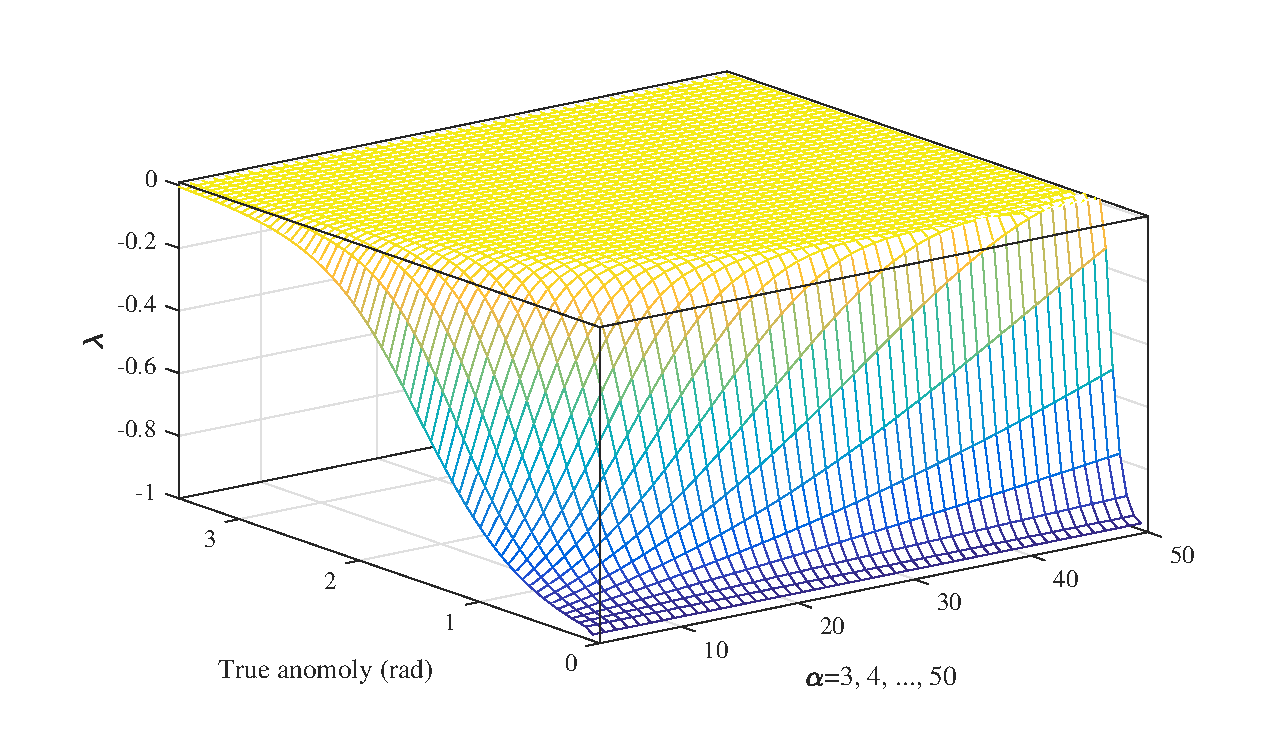
\includegraphics[width=250pt]{reducedlength.eps}  
\caption{Trajectory of tether length in reduced order system} \label{fig:graph_reduced_length}
\end{figure} 

  (2) Review Eq.(\ref{eq:lambda_k-lambda_k-1}) and rewrite it as
  \begin{align}
	  \lambda_{k} = -\left(\beta\lambda_{k-1}+\beta-1\right)\lambda_{k-1}
  \end{align}
  
  As $\lambda$ is asymptotically stable, the following inequation must hold$
	-1<\beta\lambda_{k-1}+\beta-1<1$. 
It is understood that subject to $\beta\left(\lambda_{k-1}+1\right)\in(0,2)$, increasing $\left\vert\beta\lambda_{k-1}+\beta-1\right\vert$ will degenerate the dynamic performance of tether length. Accordingly, increasing $\alpha$ will enhance the performance, which is illustrated in Figure~\ref{fig:graph_reduced_length}.


  This completes the proof.\end{proof}
  %\hfill $\blacksquare$

%\end{proof}
\subsection{Compensation analysis on tension limitation}\label{subsec:Compensation}
It is noted that tension acting on space tether is the unique driving force to govern the in-plane dynamics. If there are no bends in the space tether, as it does occur with vibrations or pulleys, then tension is a constant along the tether, equal to the magnitude of the forces applied by the reel. The reel can work like a brake to generate desired tension to tighten the tether, which guarantees the establishment of the `dumbbell' model of TSR. Hence, the tension in the tether should be a non-negative scalar quantity. 

Considering the specified relation between control law and tension $u=-\tau$, the input in Eq.(\ref{eq:control law}) should be denoted as $sat(u)$ with
\begin{align}
	sat(u)=\left\{
             \begin{array}{ll}
             u_{\max}, &u\ge u_{\max}  \\
             u, & u_{\min}<u<u_{\max}\\
             u_{\min}, &u\le u_{\min}
             \end{array}
\right.
\end{align}
where $u_{\min}<u_{\max}=-\epsilon<0$. The previous input design in Eq.(\ref{eq:control law}) only considers $sat(u)\equiv u$, which characterizes the absence of `active' input saturation with ignoring the inexistence of `negative tension', and it should be regarded as an ideal input rather than a practical command. There exists an obvious relation between practical command (limited input) $sat(u)$ and ideal input $u$ as follows:
\begin{align}
	sat(u)-u = \Delta u
\end{align}

In order to perfect the proposed discrete-time method, an auxiliary variable sequence $\chi(k)$ is introduced to weaken the impact of input saturation
\begin{align}\label{eq:chi}
	\chi(k+1)&=\left\{
             \begin{array}{ll}
             -\frac{\Lambda(k)}{\chi(k)}-(\bar\gamma-1)\chi(k), &\chi(k)>\mu   \\
             \chi(k), & \chi(k)\le \mu
             \end{array},
\right.\\
\Lambda &=\left(b\Phi_3(k)\cdot\left[\Delta u(k)+\gamma\chi(k)\right]\right)^2>0
\end{align}
where $0<\bar\gamma<1$, $\chi(0)>0$ and $\mu>0$ is a small quantity. 

The auxiliary variable sequence can be expressed by 
\begin{align}
	\chi(k+1)-\chi(k)&=\left\{
             \begin{array}{ll}
             -\frac{\Lambda(k)}{\chi(k)}-\bar\gamma\chi(k), &\chi(k)>\mu   \\
             0, & \chi(k)\le \mu
             \end{array},
\right.
\end{align}
and due to $\Lambda(k)>0$ and $\chi(k)>0$, it is a monotony decreasing sequence terminated as $0<\chi(k)\le\mu$. 

The establishment  of the proposed sliding surface can be guaranteed by the following theorem.

\begin{mythm}
Given the compensation of tension limitation, the ideal input can be designed as  
\begin{align}\label{eq:input with compensation}
	u(k) = u_{eq}(k)+u_{sw}(k)+\gamma\chi(k)
\end{align}
to drive the states onto the proposed discrete-time sliding surface in Eq.(\ref{eq:discrete time sliding furface}) although the input saturation occurs.
\end{mythm}
\begin{proof}
Introducing the input~(\ref{eq:input with compensation}) with $u_{sw}(k)=-\frac{\eta s(k)}{b\Phi_3(k)}$ into Eq.(\ref{eq:s(k+1)-s(k) s}) produces
\begin{align}\begin{split}
	&s(k+1)-s(k) \\
	&= -\eta s(k)+b\Phi_3(k)\left[\Delta u(k)+\gamma\chi(k)\right]\\
	&s(k+1)+s(k) \\
	&= -(\eta-2) s(k)+b\Phi_3(k)\left[\Delta u(k)+\gamma\chi(k)\right]
\end{split}\end{align}
Combining the two equations above gets
\begin{align}\begin{split}
	&s^2(k+1)-s^2(k) \\
	&= \eta(\eta-2)s^2(k)+b^2\Phi_3^2(k)\left[\Delta u(k)+\gamma\chi(k)\right]^2\\
	&\quad-(2\eta-2)s(k)b\Phi_3(k)\left[\Delta u(k)+\gamma\chi(k)\right]
\end{split}\end{align}
It is understood to select $\eta=1$ to enhance reaching performance by maximize the gain of $s^2(k)$ and removing the uncertain effect of $s(k)$ with $\Delta u(k)$, one can obtain
\begin{align}\begin{split}
	&s^2(k+1)-s^2(k) \\
	&\le -s^2(k)+b^2\Phi_3^2(k)\left[\Delta u(k)+\gamma\chi(k)\right]^2
\end{split}\end{align}
Considering a discrete-time Lyapunov function candidate $V(k) = s^2(k)+\chi^2(k)$, it is obvious that
\begin{align}\begin{split}\label{eq:V(k+1)-V(k)}
	&V(k+1)-V(k) \\
	&= s^2(k+1)+\chi^2(k+1)-\left[s^2(k)+\chi^2(k)\right]
\end{split}\end{align}
Because $\chi(k)$ is positive and monotony decreasing, it is understood that
\begin{align}
	\chi^2(k+1)\le\chi(k+1)\chi(k) 
\end{align}  
{\it Case} $\chi(k)>\mu$: Eq.(\ref{eq:V(k+1)-V(k)}) becomes
\begin{align}\begin{split} 
	&V(k+1)-V(k) \\
	&\le \left[s^2(k+1)-s^2(k)\right]+\chi(k)\left[\chi(k+1)-\chi(k)\right]\\
	&\le -s^2(k)+b^2\Phi_3^2(k)\left[\Delta u(k)+\gamma\chi(k)\right]^2\\
	&\quad-\chi(k)\left[\frac{\Lambda(k)}{\chi(k)}+\bar\gamma\chi(k)\right]\\
	&\le -s^2(k)+b^2\Phi_3^2(k)\left[\Delta u(k)+\gamma\chi(k)\right]^2\\
	&\quad-\Lambda(k)-\bar\gamma\chi^2(k)
\end{split}\end{align}
%In the light of $\Delta u(k)\gamma\chi(k)\le 0$, we can establish $b\Phi_3(k)\left\vert\Delta u(k)+\gamma\chi(k)\right\vert\le b\Phi_3(k)\cdot\max\left\{-\Delta u(k),\gamma\chi(k)\right\}\le\sqrt{\Lambda(k)}$ to yield
In the light of $\Lambda =\left(b\Phi_3(k)\cdot\left[\Delta u(k)+\gamma\chi(k)\right]\right)^2$, we can establish
\begin{align}\begin{split}
	V(k+1)-V(k) \le -s^2(k)-\bar\gamma\chi^2(k)\le 0
\end{split}\end{align}
Substitute Eq.(\ref{eq:V(k+1)-V(k)}) into the left side of above inequation to get
\begin{align}\begin{split}
	&s^2(k+1)+\chi^2(k+1)\\
	&\le(1-\bar\gamma)\chi^2(k)\\
	&\le(1-\bar\gamma)\left[s^2(k)+\chi^2(k)\right]\\
	&\le(1-\bar\gamma)^k\left[s^2(0)+\chi^2(0)\right]
\end{split}\end{align}
which indicates $s^2(k)+\chi^2(k)\to 0$, $k\to \infty$ with $0<1-\bar\gamma<1$.

{\it Case:} $\chi(k)\le\mu$, Eq.(\ref{eq:V(k+1)-V(k)}) becomes
\begin{align}\begin{split}
	&V(k+1)-V(k) \\
	&\le \left[s^2(k+1)-s^2(k)\right]+\chi(k)\left[\chi(k+1)-\chi(k)\right]\\
	&\le -s^2(k)+\Lambda(k)\\
	&\le -\left[s(k)+\sqrt{\Lambda(k)}\right]\left[s(k)-\sqrt{\Lambda(k)}\right]
\end{split}\end{align}
and it implies that $s(k)$ will converge into the set $\Xi=\left\{x\left\vert x<\sqrt{\Lambda}\right.\right\}$ with $k\to\infty$.

This completes the proof.\end{proof}
\begin{myrem}
	We have proved the asymptotical stability of polynomial $s^2(k)+\chi^2(k)$, and it is worth noting that it differs from that $s(k)$ and $\chi(k)$ are asymptotically stable respectively. 
	
	Particularly, this analysis has given out the conclusion that $s^2(k)+\chi^2(k)$ will converge to the origin with $k\to\infty$, but $s(k)$ and $\chi(k)$ might fluctuate as $k$ increasing, i.e., $s(k)$ might cross the origin or $\vert s(k)\vert$ increase while guaranteeing $s^2(k)+\chi^2(k)$ is decreasing. 
\end{myrem}
\begin{myrem}
	As a practically physical system, it is assumed that the ideal input $u(k)$ is bounded, and the analyses have shown that the dynamics under the tension limitation is stable. It means that there exists $\sup{\Lambda(k)},{k\in \mathbb{N}}$ with decreasing $\Phi_3(k)$. Thus it can conclude that $s(k)$ is ultimately uniformly bounded under the control input with tension limitation.
\end{myrem}

\section{Numerical Simulations}\label{sec:Numerical Simulations} 
This section will use digital computer to simulate the deployment of TSR with proposed method in previous sections to verify the analyses on stability of swinging angle and length. The sample interval is specified as $10$ ms to test the performance of proposed discrete-time method in digital computer environment. 

The parameters and initial conditions of deployment mission are listed. The physical parameters are total length of tether $L=3.5$  km, equivalent mass of system $\bar m=10$ kg, orbital velocity $\Omega = 0.00117$ rad/s. The initial conditions are as follows: $\lambda_0=-0.975$, $\lambda_1=-0.97499298$, $\theta_0=\theta_1=0.1$ rad~\cite{williams2008deployment}. Controller parameters are selected according to different cases as follows:

In the case of input without saturation compensation (\ref{eq:chi}), $c_1=5.20$, $c_2=10.51$, $\alpha=3.50$ and $\eta=0.5$, these parameters meet the requirements mentioned in stability analyses, and moreover, the input saturation has been carefully avoided actively with these appropriate parameters selected. 

The controller parameters are easier to choose in the case of input with saturation compensation (\ref{eq:chi}), and we determine the controller with $c_1=1.92$, $c_2=6.22$, $\alpha=3.50$ and $\eta=1$. The auxiliary parameters are selected as $\chi(0) = 3$, $\gamma = 1\times 10^{-3}$, $\bar\gamma = 1\times 10^{-4}$, $\mu=0.1$ to keep $\chi$ working for a considerable time so that $s^2+\chi^2$ can perform asymptotical convergence. The input boundary can be described by $u_{\max} = 0$ and $u_{\min} = -0.2875$ meaning that the tension is subject to the condition $0<\tau<0.2875 N$.
In addition, the continuous switching input is adopted in this simulations.

\begin{figure}[htbp]
\centering
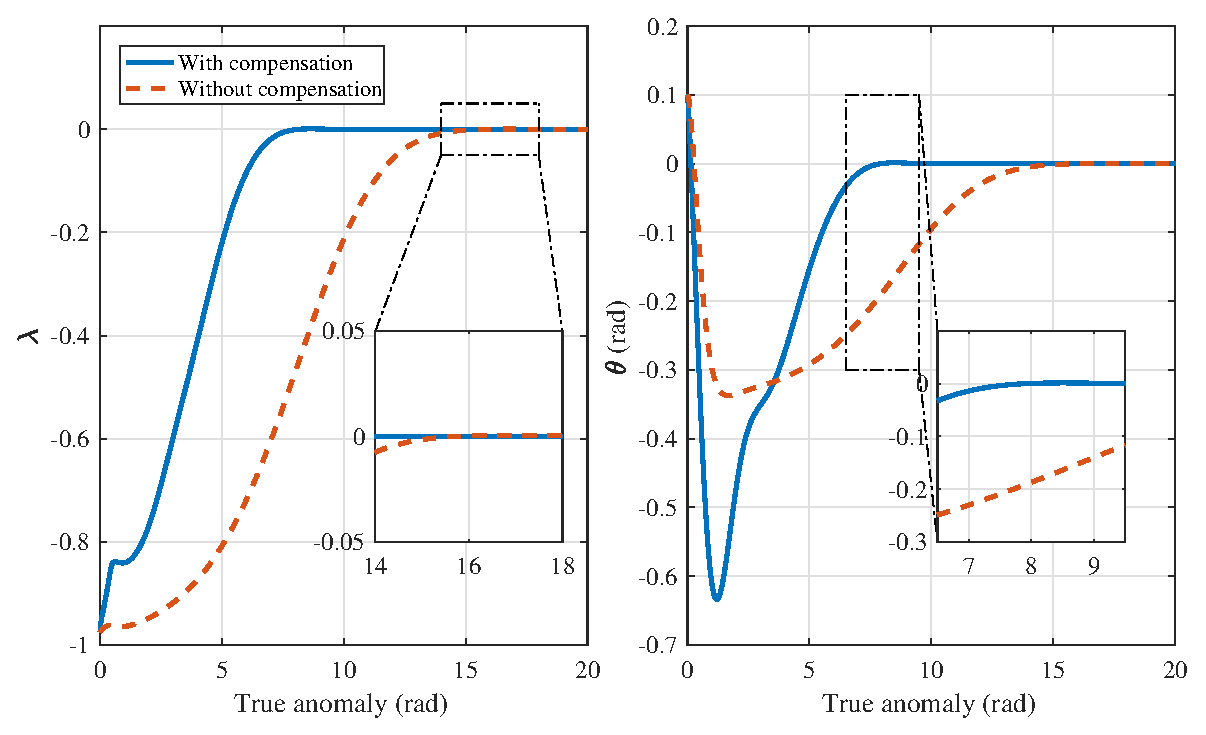
\includegraphics[width=250pt]{tether.eps}
\caption{Trajectory of tether length and swinging angle} \label{fig:graph_tether}
\end{figure}

Simulation results are illustrated from Figure~\ref{fig:graph_tether} to \ref{fig:graph_chi} including the trajectories of tether length, swinging angle, sliding mode dynamics, reduced order  system dynamics on the sliding surface, input and auxiliary variable. Figure~\ref{fig:graph_tether} shows the trajectory of tether length and swinging angle, respectively. In the case without the input saturation compensation, controller parameters are selected carefully in aid of the input locating in the linear part rather than the saturation. As a result, one can find that the deployment mission completes at true anomaly 16 rad when the length and angle both converge to the origin, and the entire deployment is smooth and flat. 

The simulation results have verified that the DSMC strategy can stabilize the deployment dynamics of TSR, but due to the physical tension limitation, it is hard to select appropriate parameters for better performance, i.e., the controller parameters corresponding to a fast deployment always lead to unattainable inputs (`negative' tension). Hence, we synthesize this method and the auxiliary sequence to actively generate saturated inputs to liberate the selection of controller parameters. It performs a fast deployment which is characterized by high-quality dynamics of length and large swinging angle. From the results in Figure~\ref{fig:graph_tether}, the mission completes in true anomaly 9 rad faster than the one without the compensation. 

These simulation results above are coincident with the stability analyses and verify the controller design for the fast deployment of TSR. It is worth noting that this work is dependent on a digital control strategy without velocity sensor and estimator, and the considerable length and angle resolution is required correspondingly. We take a big sample interval in this mission, which does not affect the stability of the proposed DSMC strategy. Besides the advantages mentioned above, a fast deployment can be achieved based on DSMC with the compensation. 

\begin{figure}[htbp] 
\centering
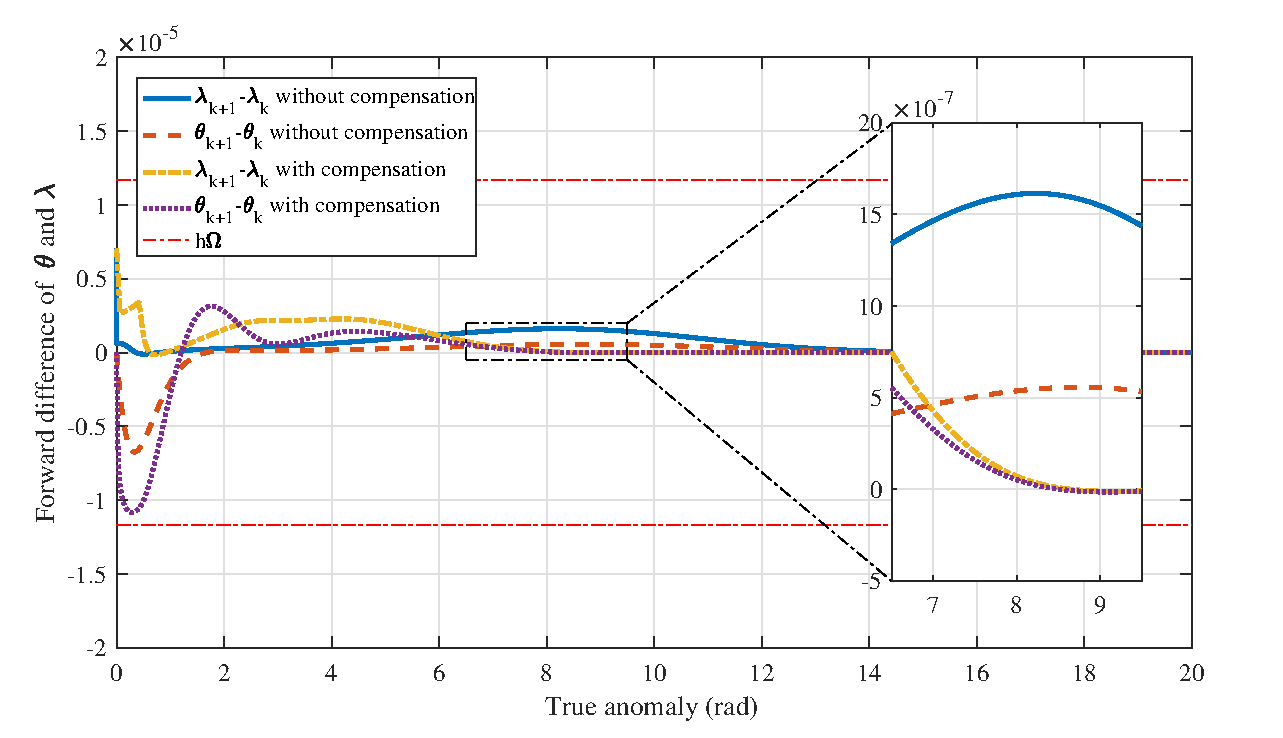
\includegraphics[width=250pt]{forwarddifference.eps}
\caption{Trajectory of forward difference of length and swinging angle} \label{fig:graph_diff}
\end{figure}

On the basis of results shown in Figure~\ref{fig:graph_tether}, Figure~\ref{fig:graph_diff} illustrates the forward difference of length and swinging angle. From the results, length difference practically locates in the value region of $10^{-6}$, and considering the total length $L=3.5$ km in this mission, it requires the length's measurement precision of $10^{-3} $ m that is easy to meet for industrial length sensors. Similarly, it is also easy to meet the angle's measurement precision for industrial angle sensors. The red point lines denote the valid boundary of swinging angle's difference to avoid the singularity of input caused by $\Phi_3=0$, and if the trajectory of forward difference is very close to boundary, it will ruin the control strategy. 

In the enlarged figure, states of DSMC with compensation sustain converging to the origin in the value level of $10^{-7}$ around true anomaly 8.5 rad, which is coincident with the analyses in controller design. This indicates the analyses in Remark~\ref{rem:2} are convincing. The forward difference of DSMC without compensation converge to the origin after true anomaly 14 rad, which can also be observed from the trajectories in Figure~\ref{fig:graph_tether}. Moreover, these trajectories reflect the increment fluctuation, a flat trajectory results in a smooth deployment dynamics corresponding to the DSMC without the compensation, whereas the monotone increment trajectory indicates that a magnitude state is produced such as the swinging angle under the DSMC with the compensation.

\begin{figure}[htbp] 
\centering
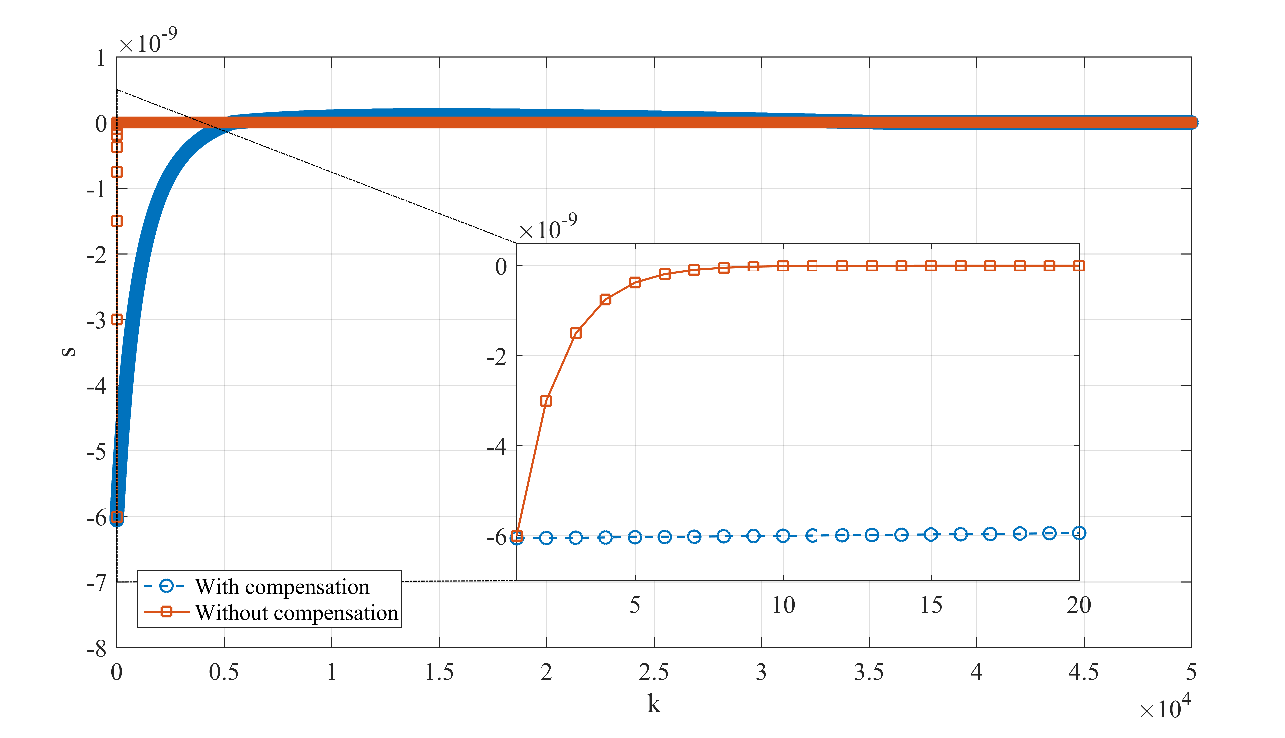
\includegraphics[width=250pt]{slidingsurface.eps}
\caption{Trajectory of sliding surface variable} \label{fig:graph_s}
\end{figure} 

Figure~\ref{fig:graph_s} illustrates the trajectory of sliding surface variable. From the simulation results, under the DSMC, it can be found that in the case without the compensation, the performance of sliding surface variable is characterized by asymptotical convergence to the origin. The trajectory in the case with compensation rise slowly, because the convergence speed is determined by the switching input which is actively affected by the saturation. This occasion directly degenerates the reaching performance, which is evaluated by the convergence coefficient $(1-\bar\gamma)^k$ in Section~\ref{subsec:Compensation}, although the coefficient is very conservative. It is an important matter that $\chi>\mu$ should be maintained to sustain the asymptotical convergence of $s^2+\chi^2$, hence $\bar\gamma = 1\times 10^{-4}$ is chosen such that $\chi$ will not enter the set $\{x\vert 0<x<\mu\}$ too early. From Figure~\ref{fig:graph_s}, it is after 5000 steps the sliding mode variable $s$ crosses the origin triggering an obvious overshoot, and then $s$ falls back to the origin around $4\times 10^4$ steps. Before explaining this circumstance, it is meaningful to recognize the difference between the asymptotical convergence of $s^2+\chi^2$ and that of $s$ and $\chi$ respectively. For $t\to\infty$, in the view of the results $s\to 0$ and $\chi\to 0$, these two scenarios seem the same. However, if we carefully check the processing of $s^2+\chi^2\to 0$, which allows the fluctuation of state, and this is the reason why an overshoot of $s$ can be seen.  After $s$ reaching the origin or its vicinity $\Theta=\{x\vert 0<x<\epsilon\}$,  the switching input prevents the sliding mode variable $s$ escaping from $\Theta$, and the reduced order  system hence exists and governs the entire dynamics. Proposed sliding surface can make a specified reduced order  system that states are asymptotically stable at the origin.  

\begin{figure}[htbp] 
	\centering
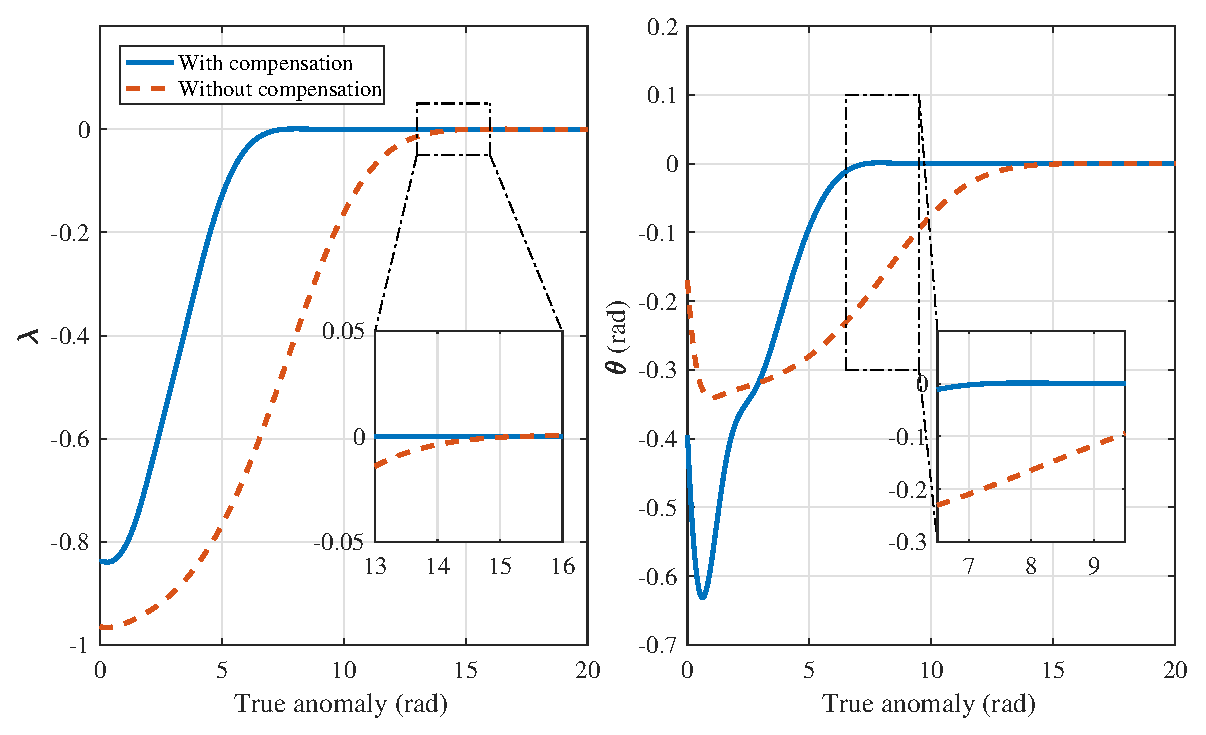
\includegraphics[width=250pt]{reducedsystem.eps}
\caption{Trajectory of tether length and swinging angle of reduced order  system} \label{fig:graph_reduced_system}
\end{figure} 

In this dimensionless discrete-time system, $k=5\times 10^4$ equals to true anomaly $5\times 10^4h\Omega=0.584 $ rad. Figure~\ref{fig:graph_reduced_system} plots the trajectories of reduced order  dynamics, the simulation is initialized by the status at 0.584 rad in the original system, for the case with compensation $\lambda_0 =-0.8387322$, $\lambda_1 =-0.8387320$, $\theta_0 =-0.395875$ and $\theta_1 =-0.395884$; for the case without compensation $\lambda_0 =-0.9643726$, $\lambda_1 =-0.9643727$, $\theta_0 =-0.170058$ and $\theta_1 =-0.170064$. Combining with the results in Figure~\ref{fig:graph_s}, we can find that the motion dynamics with compensation on the sliding surface is much better than that without compensation, and the final stability time is approximately the sum of reaching time and sliding time. Furthermore, one can image that the trajectories without compensation are triggered with the same initial status by left shifting, and the results will not change. 
 
\begin{figure}[htbp] 
	\centering
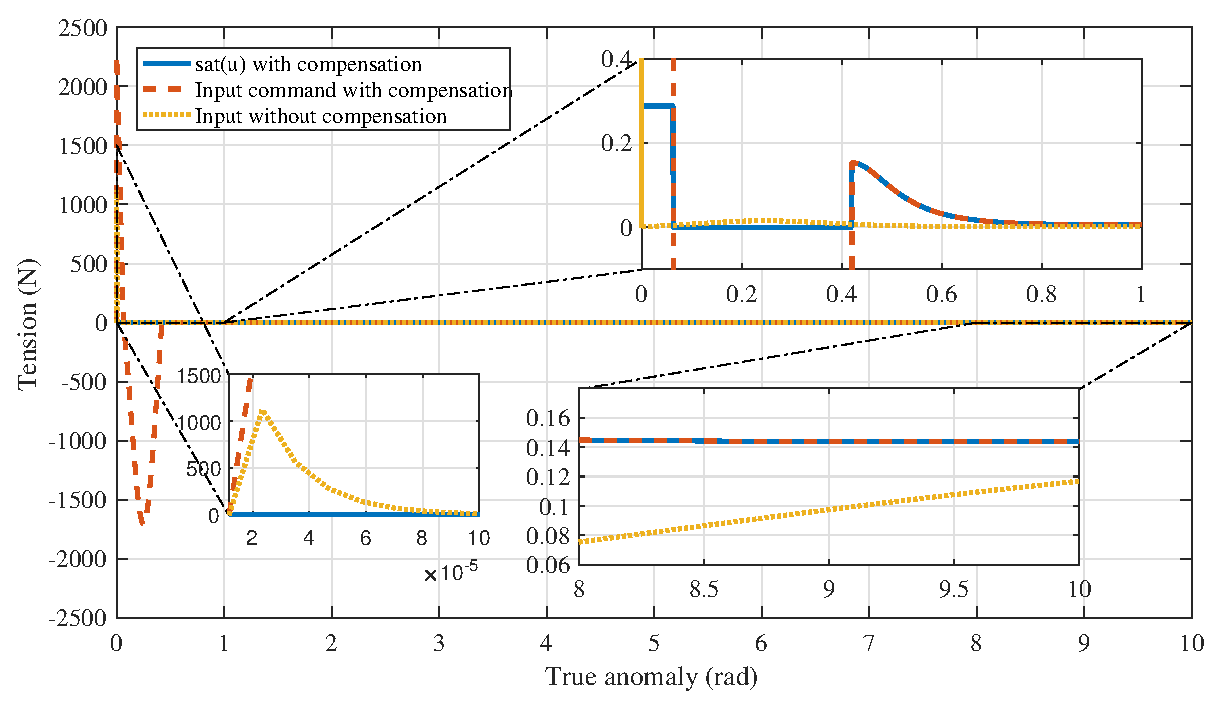
\includegraphics[width=250pt]{input.eps}
\caption{Trajectory of input} \label{fig:graph_input}
\end{figure} 

% illustrate the fact
Figure~\ref{fig:graph_input} gives out the simulation results of inputs.
% describe the formation
From the trajectory of input without compensation, one can find there is not negative tension generated due to the carefully selection of parameters, but there is a sharp rise over 1000 N at the beginning of deployment mission. Based on the previous stability analysis, this input guarantees the reaching condition of sliding surface, while it is worth noting that when the deployment stabilized, the input is between 0.14 to 0.16 N. In other words, this control scheme requires a resolution over $0.1\%$ with a measurement range of 1000 N. 
% analyze the effect of disadvantage
With the compensation aided, the controller parameters can be widely selected from the premise that the control system is stabilized. From Figure~\ref{fig:graph_input} , it is clear that the actual inputs are saturated in a preset range from 0 to 0.4 true anomaly, although the input commands are badly over the preset range. 
% comparison
Combining with the results in Figure~\ref{fig:graph_diff} and Figure~\ref{fig:graph_tether}, the input with compensation changed suddenly especially around 0.4 true anomaly, while the counterpart is much flatter, this is because that the rapidly changing is blocked by the large tension over 1000 N at the beginning.  
% explain the reason of advantage
From the selection of tension sensor or generator, the method with compensation only requires a trivial one with the range of 1 N and the resolution of $1\%$. 

It is worth noting that the trajectory of ${\rm sat}(u)$ shows the actual tension acting on the tether, and the corresponding input command before the ${\rm sat}()$ model is denoted as `input command with compensation'. Hence it is clear to find that these two trajectories are coincident if there is no saturation. Similar to the input denoted as  ${\rm sat}(u)$, it is required that input without compensation should directly act on the tension control of space tether, so the control parameters are well selected to make it satisfy the condition of not crossing the limitation of maximum/minimum tension. For this purpose, a slow deployment can be found as the discussion in Fig~\ref{fig:graph_tether}. Considering the issue of input with compensation, the fluctuation of input command is not a matter that has to be coped with, since the actual input is always physically meaningful due to the existence of input saturation and compensation. The fluctuation of input command is caused by the loose selection of controller parameters, which is one of the advantage of proposed compensation method.
\begin{figure}[htbp]  
	\centering
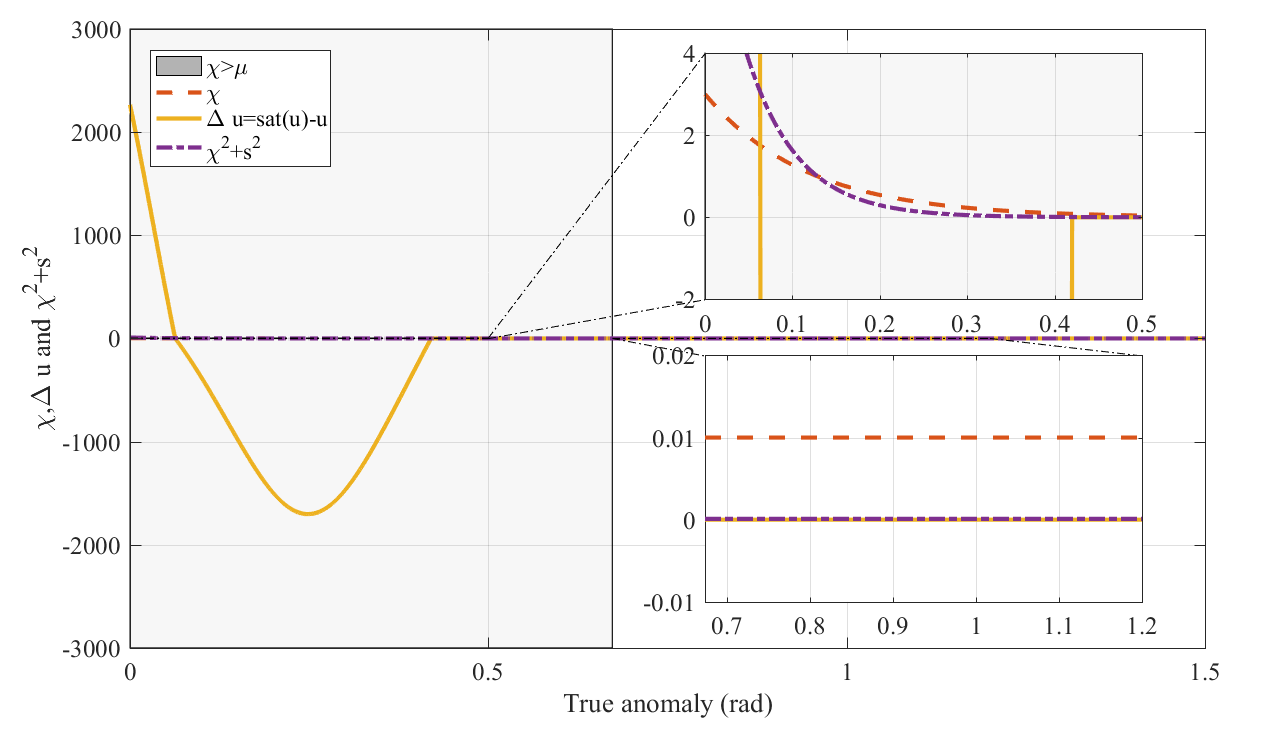
\includegraphics[width=250pt]{chi.eps}
\caption{Trajectory of $\chi$, $\chi^2+s^2$ and $\Delta u$} \label{fig:graph_chi}
\end{figure} 

Figure~\ref{fig:graph_chi} shows the relation between inputs, commands and auxiliary variables. The gray region denotes the `legal' range of input saturation, meaning the theoretical stability of control system can be rigorously guaranteed. Once the trajectory leaves this region, the stability character turns the uniform boundedness from asymptotical stability. The results in the figure indicate all the input saturations occur in the gray range, namely, before the auxiliary variable invalided. The results are in accordance with the previous stability analyses in this paper.  
\section{Conclusion}
This paper presents a nonlinear discrete-time sliding mode based tension control technique for deployment of TSR with only length and angle measurements. The main contribution of this work is to propose a new nonlinear discrete-time sliding surface for generating a specified reduced order  system, and the motion of swinging angle and length on the sliding surface is robust stable and asymptotically stable, respectively. A novel discrete-time compensation works to guarantee the establishment of sliding surface although input saturation occurs. A considerable sample interval is used in the mission, and simulation results indicate that proposed method does not require high-precision length and angle sensors to be implemented, which may aid the future astronautic experiments and applications. 


%张力过大容易破坏reel,文中没有指出。


% if have a single appendix:
%\appendix[Proof of the Zonklar Equations]
% or
%\appendix  % for no appendix heading
% do not use \section anymore after \appendix, only \section*
% is possibly needed

% use appendices with more than one appendix
% then use \section to start each appendix
% you must declare a \section before using any
% \subsection or using \label (\appendices by itself
% starts a section numbered zero.)
%


%\appendices
%\section{Proof of the First Zonklar Equation}
%Appendix one text goes here.

% you can choose not to have a title for an appendix
% if you want by leaving the argument blank
%\section{}
%Appendix two text goes here.


% use section* for acknowledgment
%\section*{Acknowledgment}


%The authors would like to thank...


% Can use something like this to put references on a page
% by themselves when using endfloat and the captionsoff option.
\ifCLASSOPTIONcaptionsoff
  \newpage
\fi



% trigger a \newpage just before the given reference
% number - used to balance the columns on the last page
% adjust value as needed - may need to be readjusted if
% the document is modified later
%\IEEEtriggeratref{8}
% The "triggered" command can be changed if desired:
%\IEEEtriggercmd{\enlargethispage{-5in}}

% references section

% can use a bibliography generated by BibTeX as a .bbl file
% BibTeX documentation can be easily obtained at:
% http://mirror.ctan.org/biblio/bibtex/contrib/doc/
% The IEEEtran BibTeX style support page is at:
% http://www.michaelshell.org/tex/ieeetran/bibtex/
%\bibliographystyle{IEEEtran}
% argument is your BibTeX string definitions and bibliography database(s)
%\bibliography{sample}
% Generated by IEEEtran.bst, version: 1.14 (2015/08/26)
\begin{thebibliography}{10}
	\providecommand{\url}[1]{#1}
	\csname url@samestyle\endcsname
	\providecommand{\newblock}{\relax}
	\providecommand{\bibinfo}[2]{#2}
	\providecommand{\BIBentrySTDinterwordspacing}{\spaceskip=0pt\relax}
	\providecommand{\BIBentryALTinterwordstretchfactor}{4}
	\providecommand{\BIBentryALTinterwordspacing}{\spaceskip=\fontdimen2\font plus
	\BIBentryALTinterwordstretchfactor\fontdimen3\font minus
		\fontdimen4\font\relax}
	\providecommand{\BIBforeignlanguage}[2]{{%
	\expandafter\ifx\csname l@#1\endcsname\relax
	\typeout{** WARNING: IEEEtran.bst: No hyphenation pattern has been}%
	\typeout{** loaded for the language `#1'. Using the pattern for}%
	\typeout{** the default language instead.}%
	\else
	\language=\csname l@#1\endcsname
	\fi
	#2}}
	\providecommand{\BIBdecl}{\relax}
	\BIBdecl
	
	\bibitem{yu2018review}
	B.~Yu, H.~Wen, and D.~Jin, ``Review of deployment technology for tethered
		satellite systems,'' \emph{Acta Mechanica Sinica}, pp. 1--15, 2018.
	
	\bibitem{ma2017dynamic}
	Z.~Ma, G.~Sun, and Z.~Li, ``Dynamic adaptive saturated sliding mode control for
		deployment of tethered satellite system,'' \emph{Aerospace Science and
		Technology}, vol.~66, pp. 355--365, 2017.
	
	\bibitem{wang2015coordinated}
	D.~Wang, P.~Huang, and Z.~Meng, ``Coordinated stabilization of tumbling targets
		using tethered space manipulators,'' \emph{IEEE Transactions on Aerospace and
		Electronic Systems}, vol.~51, no.~3, pp. 2420--2432, 2015.
	
	\bibitem{Zhang2017}
	F.~Zhang and P.~Huang, ``{Releasing Dynamics and Stability Control of
		Maneuverable Tethered Space Net},'' \emph{IEEE/ASME Transactions on
		Mechatronics}, vol.~22, no.~2, pp. 983--993, 2017.
	
	\bibitem{Zhang2017JGCD}
	F.~Zhang, P.~Huang, Z.~Meng, Y.~Zhang, and Z.~Liu, ``{Dynamics Analysis and
		Controller Design for Maneuverable Tethered Space Net Robot},'' \emph{Journal
		of Guidance, Control, and Dynamics}, vol.~40, no.~11, pp. 1--16, 2017.
	
	\bibitem{Huang2017}
	P.~Huang, F.~Zhang, J.~Cai, D.~Wang, Z.~Meng, and J.~Guo, ``{Dexterous Tethered
		Space Robot: Design, Measurement, Control, and Experiment},'' \emph{IEEE
		Transactions on Aerospace and Electronic Systems}, vol.~53, no.~3, pp.
		1452--1468, 2017.
	
	\bibitem{dai2018post}
	H.~Dai, X.~Jing, Y.~Wang, X.~Yue, and J.~Yuan, ``Post-capture vibration
		suppression of spacecraft via a bio-inspired isolation system,''
		\emph{Mechanical Systems and Signal Processing}, vol. 105, pp. 214--240,
		2018.
	
	\bibitem{liu2017tether}
	H.~Liu, Y.~He, H.~Yan, and S.~Tan, ``Tether tension control law design during
		orbital transfer via small-gain theorem,'' \emph{Aerospace Science and
		Technology}, vol.~63, pp. 191--202, 2017.
	
	\bibitem{yu2017analytical}
	B.~Yu, D.~Jin, and H.~Wen, ``An analytical control law of length rate for
		tethered satellite system,'' \emph{Meccanica}, vol.~52, no.~9, pp.
		2035--2046, 2017.
	
	\bibitem{ma2018pure}
	Z.~Ma, G.~Sun, Z.~Cheng, and Z.~Li, ``Pure-tension non-linear sliding mode
		control for deployment of tethered satellite system,'' \emph{Proceedings of
		the Institution of Mechanical Engineers, Part G: Journal of Aerospace
		Engineering}, vol. 232, no.~13, pp. 2541--2551, 2018.
	
	\bibitem{williams2008deployment}
	P.~Williams, ``Deployment/retrieval optimization for flexible tethered
		satellite systems,'' \emph{Nonlinear dynamics}, vol.~52, no. 1-2, pp.
		159--179, 2008.
	
	\bibitem{wen2008optimal}
	H.~Wen, D.~Jin, and H.~Hu, ``Optimal feedback control of the deployment of a
		tethered subsatellite subject to perturbations,'' \emph{Nonlinear Dynamics},
		vol.~51, no.~4, pp. 501--514, 2008.
	
	\bibitem{Kang2018}
	J.~Kang, Z.~H. Zhu, A.~Li, C.~Wang, and W.~Wang, ``{Energy-based Output
		Feedback Tension Control for Space Tether Deployment under Physical
		Constraint},'' \emph{Proceedings of the American Control Conference}, vol.
		2018-June, pp. 646--651, 2018.
	
	\bibitem{zhang2017adaptive}
	Y.~Zhang and Q.~Xu, ``Adaptive sliding mode control with parameter estimation
		and kalman filter for precision motion control of a piezo-driven
		microgripper,'' \emph{IEEE Transactions on Control Systems Technology},
		vol.~25, no.~2, pp. 728--735, 2017.
	
	\bibitem{sun2018discrete}
	G.~Sun, Z.~Ma, and J.~Yu, ``Discrete-time fractional order terminal sliding
		mode tracking control for linear motor,'' \emph{IEEE Transactions on
		Industrial Electronics}, vol.~65, no.~4, pp. 3386--3394, 2018.
	
	\bibitem{Nohmi2009}
	M.~Nohmi, ``{Mission design of a tethered robot satellite `STARS' for orbital
		experiment},'' \emph{2009 IEEE Control Applications, (CCA) {\&} Intelligent
		Control, (ISIC)}, pp. 1075--1080, 2009.
	
	\bibitem{Gates2001}
	S.~Gates, S.~Koss, and M.~Zedd, ``{Advanced Tether Experiment Deployment
		Failure},'' \emph{Journal of Spacecraft and Rockets}, vol.~38, no.~1, 2001.
	
	\bibitem{Iki2014}
	K.~Iki, S.~Kawamoto, and Y.~Morino, ``{Experiments and numerical simulations of
		an electrodynamic tether deployment from a spool-type reel using
		thrusters},'' \emph{Acta Astronautica}, vol.~94, no.~1, pp. 318--327, 2014.
	
	\bibitem{Nakaya2004}
	K.~Nakaya, M.~Iai, K.~Omagari, H.~Yabe, and S.~Matunaga, ``{Formation
		Deployment Control for Spinning Tethered Formation Flying - Simulations and
		Ground Experiments},'' \emph{AIAA Guidance, Navigation, and Control
		Conference and Exhibit}, no. August, pp. 2--12, 2004.
	
	\bibitem{Bloch2005Controlled}
	A.~M. Bloch, M.~Leok, J.~E. Marsden, and D.~V. Zenkov, ``Controlled lagrangians
		and stabilization of the discrete cart-pendulum system,'' in
		\emph{Proceedings of the 44th IEEE Conference on Decision and Control}, Dec
		2005, pp. 6579--6584.
	
	\bibitem{Marsden2001Discrete}
	J.~E. Marsden and M.~West, ``Discrete mechanics and variational integrators,''
		\emph{Acta Numerica}, vol.~10, pp. 357--514, 2001.
	
	\bibitem{Xu2008}
	R.~Xu and {\"{U}}.~{\"{O}}zg{\"{u}}ner, ``{Sliding mode control of a class of
		underactuated systems},'' \emph{Automatica}, vol.~44, no.~1, pp. 233--241,
		2008.
	
	\bibitem{Gao2004}
	H.~Gao and C.~Wang, ``Delay-dependent robust stabilization for uncertain
		discrete-time systems with multiple state delays,'' \emph{Acta Automatica
		Sinica}, vol.~30, no.~5, pp. 789--795, Sep. 2004.
	
	\end{thebibliography}
	
%
% <OR> manually copy in the resultant .bbl file
% set second argument of \begin to the number of references
% (used to reserve space for the reference number labels box)
%\begin{thebibliography}{1}

%\bibitem{IEEEhowto:kopka}
%H.~Kopka and P.~W. Daly, \emph{A Guide to \LaTeX}, 3rd~ed.\hskip 1em plus
%  0.5em minus 0.4em\relax Harlow, England: Addison-Wesley, 1999.

%\end{thebibliography}

% biography section
% 
% If you have an EPS/PDF photo (graphicx package needed) extra braces are
% needed around the contents of the optional argument to biography to prevent
% the LaTeX parser from getting confused when it sees the complicated
% \includegraphics command within an optional argument. (You could create
% your own custom macro containing the \includegraphics command to make things
% simpler here.)
%\begin{IEEEbiography}[{\includegraphics[width=1in,height=1.25in,clip,keepaspectratio]{mshell}}]{Michael Shell}
% or if you just want to reserve a space for a photo:

%\begin{IEEEbiography}{Michael Shell}
%Biography text here.
%\end{IEEEbiography}

% if you will not have a photo at all:
%\begin{IEEEbiographynophoto}{John Doe}
%Biography text here.
%\end{IEEEbiographynophoto}

% insert where needed to balance the two columns on the last page with
% biographies
%\newpage

%\begin{IEEEbiographynophoto}{Jane Doe}
%Biography text here.
%\end{IEEEbiographynophoto}

% You can push biographies down or up by placing
% a \vfill before or after them. The appropriate
% use of \vfill depends on what kind of text is
% on the last page and whether or not the columns
% are being equalized.

%\vfill

% Can be used to pull up biographies so that the bottom of the last one
% is flush with the other column.
%\enlargethispage{-5in}
\begin{IEEEbiography}[{
\includegraphics[width=1in,height=1.25in]{zqma}}]{Zhiqiang Ma (S'14-M'18)}
	%\begin{IEEEbiographynophoto}{Zhiqiang Ma (S'14-M'18)}
		%Biography text here.
		 received the B.S. degree and the M.S. degree in control engineering from Northwestern Polytechnical University, China, in 2011 and 2014, and the Ph.D. degree in control science and engineering from Harbin Institute of Technology, China, in 2018, respectively. He is currently an Associate Professor of the School of Astronautics at Northwestern Polytechnical University, China. His current research interests include nonlinear dynamics and control, space tethered system, teleoperation systems and mechatronics.
		
		\end{IEEEbiography}
	\begin{IEEEbiography}[{
\includegraphics[width=1in,height=1.25in]{pfhuang}}]{Panfeng Huang (S'01-M'05-SM'17)}
	%\begin{IEEEbiographynophoto}{}
	%Biography text here.
	 received the B.S. and M.S. degrees in test and measurement technology, and navigation guidance and control from Northwestern Polytechnical University, Xi¡¯an, China, in 1998 and 2001, respectively, and the Ph.D. degree in the area of automation and robotics from the Chinese University of Hong Kong, Hong Kong, in 2005. He is currently a Professor with the School of Astronautics, Northwestern Polytechnical University, and the National Key Laboratory of Aerospace Flight Dynamics, and the Vice Director of the Research Center for Intelligent Robotics at the Northwestern Polytechnical University. His research interests include tethered space robotics, intelligent control, machine vision, and space teleoperation.
	
	\end{IEEEbiography}


% that's all folks
\end{document}


